\section*{Exercise Part (B) - A Simple Stream Cipher}

\begin{enumerate}[wide, label=(B\arabic*)]

% B1 Pick any image you like from the www, and save it to a file. You can crop the image, to  make it smaller and easier to work with. Read the image into matlab, to create a bit-map image, ie try “A = imread(my_image.png)” or “A = imread(my_image.jpg)”.
% According to Matlab documentation, the bit-map image A is a 3D array with R rows, C columns, and a depth of 3 numbers. Each number is between 0 and 255, and represents a color intensity (for 3 colors R,G,B). You can view the image in matlab with “image(A)”. Show the image in your lab report. 
% (My version of Matlab is inconsistent: A is sometimes read as a 2D matrix, and sometimes read as a 3D matrix. To make Matlab realize A is a 3D matrix, type and execute these lines: R_matrix = A(:,:,1); G_matrix = A(:,:,2); B_matrix = A(:,:,3); Thereafter, if you call “[rows,cols,depth] = size(A)”, and Matlab should view A as a 3D matrix.)
\item
For this experiment, we used an image of Dimorphos taken from the recent NASA DART mission. The image can be seen in Figure~\ref{fig:B1}. This image was downloaded from the internet, resized to a size of 418x418 using the Image Resizer utility from Microsoft PowerToys. As the LSFR in Exercise A produces 4194303 random bits, or 524288 bytes when we store it in `\texttt{my\_random\_numbers.m}', we can only use pictures that contain 174762 ($524288 / 3$ random numbers for each R, G, B value for each pixel) or less pixels, which is approximately 418x418 if the image is a square. This image was read into MATLAB using the built-in \texttt{imread} function, storing the image and it's bit-map into the 3D matrix \texttt{A}. 
\begin{figure}[htp]
    \centering
    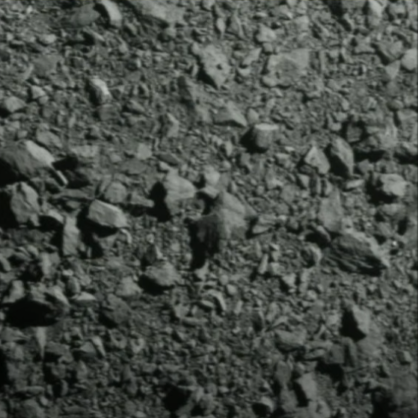
\includegraphics[width=0.7\textwidth]{dimorphos.png}
    \caption{\label{fig:B1}Image of Dimorphos from NASA DART spacecraft}
\end{figure}

% B2 Read the stream of pseudo-random numbers from the LFSR, that you wrote to a file in part A3. Write the numbers into a matrix RAND_matrix, with the same size as the A matrix. (Recall that you wrote your random numbers to a matlab file in part A3. Call that script in your matlab code, to load those numbers into your memory.) If you do not have enough random numbers, then we really should use a larger LFSR. However, to simplify lab. #1 you can also re-use some of the same random numbers. (This of course invalidates Shannon’s “One-Time-PAD” principle, and makes the cipher very weak.) You can create a 3D matrix of zeros called RAND_matrix with the command RAND_matrix = zeros(rows,cols,depth);
% You can then write your LFSR numbers into the RAND_matrix.
% Explain how you did part B2 in your lab report.
\item
The stream of pseudo-random numbers from the LFSR was read in by calling the `\texttt{my\_random\_numbers.m}' script which stored these random decimal numbers. Once the script has loaded the random numbers, we create \texttt{RAND\_matrix} with the following command:\\
\texttt{RAND\_matrix = RANDOM\_DATA\_OUT(1:numel(A));}
\\We generate this matrix by just taking the same number of random numbers from the stored matrix as we have in the matrix bit-map of the image we read in A1. We do not create \texttt{RAND\_matrix} as a 3D matrix as it is not necessary for our operations in the following steps.

% B3 You need to XOR the 3D matrix A with a 3D matrix of random numbers RAND_matrix, to encrypt the matrix A. I did this as follows: Visit each element of A and the corresponding element of RAND_matrix. These elements are decimal integers between 0 and 255. You can convert each of them to a vector of 8 bits, XOR the two bit vectors, and convert the resulting bit- vector back unto a decimal number. Write that decimal number into the element A_encrypted. You can try other ways in Matlab, to accomplish this XOR functionality too. Explain how you accomplish part B3 in your lab report.
\item
We create the uint8 matrix \texttt{A\_encrypted} in MATLAB with the same size and dimensions of \texttt{A}, which stores the image we read in. To perform the XOR operation, we iterate through all the elements of \texttt{A} and \texttt{RAND\_matrix} accessing each element by their index, and performing a bitwise XOR operation using MATLAB's built-in \texttt{bitxor} function with the following command:\\
\texttt{A\_encrypted(i) = bitxor(A(i), RAND\_matrix(i));}

% B4 View the encrypted image, using the matlab image command. Convert the matrix A_encrypted to unsigned 8 bit integers. Use the following command:
% image (uint8(A_encrypted))
% It should appear to be “random noise”. Show the image in your lab report.
\item
As the matrix \texttt{A\_encrypted} is already of the type uint8, we can view the image without conversion by using the \texttt{image} function. The encrypted image can be seen in Figure~\ref{fig:B4}. The image appears to be random noise as expected.
\begin{figure}[htp]
    \centering
    
\includegraphics[width=0.7\textwidth]{encrpyted_image.png}
    \caption{\label{fig:B4}Encrypted Image}
\end{figure}

% B5 Decrypt the ciphertext, by XOR-ing the encrypted image matrix with the random matrix used for encryption. (Do the reverse process from what was described in B3.) View the decrypted image, using the following command:
% image (uint8(A_decrypted))
% You should see the original image. Explain how you did part B5 in your lab report.
% Show the image in your lab report.
\item
Similar to the process described in A3, We create the uint8 matrix \texttt{A\_decrypted} in MATLAB with the same size and dimensions of \texttt{A\_encrypted}. To perform the XOR operation, we iterate through all the elements of \texttt{A\_encrypted} and \texttt{RAND\_matrix} accessing each element by their index, and performing a bitwise XOR operation using MATLAB's built-in \texttt{bitxor} function with the following command:\\
\texttt{A\_decrypted(i) = bitxor(A\_encrypted(i), RAND\_matrix(i));}\\
As the matrix \texttt{A\_decrypted} is already of the type uint8, we can view the image without conversion by using the \texttt{image} function. The encrypted image can be seen in Figure~\ref{fig:B5}. The image appears to match the original image in Figure~\ref{fig:B1} as expected.
\begin{figure}[htp]
    \centering
    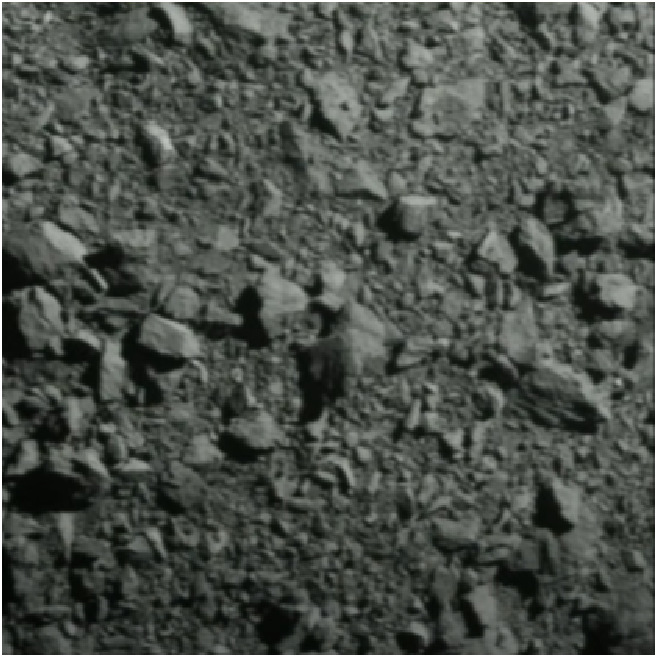
\includegraphics[width=0.7\textwidth]{decrypted_image.png}
    \caption{\label{fig:B5}Decrypted Image}
\end{figure}

% B6
% Ideally, your software will be general, ie you can view any image from the web, save it to a file, and crop it. You then run your software: view the image in Matlab, then encrypt it, view the encrypted image in Matlab, then decrypt it, and view the decrypted image in Matlab. You should only need to enter a file name, to read the original image file. The software should do the rest.
\item
The script was modified to take an image of any size so that the user does not need to crop it. When inputting an image with too many pixels, the script will prompt the user asking if they wish to resize it to 418x418, resizing the image and proceeding with the processes described above if they accept and exiting the script otherwise. To select the input image, the user simply needs to change the variable \texttt{image\_path} to the path of the image relative to the location of the script, and run the script.

\end{enumerate}